%\section{Systemmodelle}
\newpage
\subsection{Anwendungsfalldiagramm}
Das System ist in die Benutzer*gruppen \emph{Benutzer*}, \emph{Betreuer*} und \emph{Administrator*} unterteilt. Folgendes Use-Case-Diagramm beschreibt die Interaktionsmöglichkeiten der einzelnen Benutzer*gruppen mit dem Server:
\begin{itemize}
	\item Mit dem Accounts Verwalten kann der \emph{Administrator*} neuen \emph{Benutzer*} anlegen, Account abändern, Rechte vergeben oder löschen.
	\item Mit Komponente Login können \emph{Benutzer*} sich anmelden bzw. abmelden.
	\item Eine \emph{Benutzer*} kann neue Zeiterfassung starten. Nachträgliche Erfassung, Bearbeitung oder Korrektur ist möglich. Er darf seine eigene erfasste Zeiten und \emph{Stundenzettel} ansehen. Er kann Warnungen und Erinnerungen lesen. Er druckt sein \emph{Stundenzettel} aus, unterschreibt und gibt es bei seinem \emph{Betreuer*} ab.
	\item \emph{Betreuer*} darf die Erfasste Zeiten, \emph{Stundenzettel}, und Nachrichten von allen seinen zugewiesenen \emph{Benutzer*} ansehen. Er kontrolliert \emph{Stundenzettel} von seinen \emph{Benutzer*} und gibt die Status weiter an den \emph{Administrator*}.
	\item Der \emph{Administrator*} darf alles ansehen. Außerdem sammelt er noch alle \emph{Stundenzettel} ein.
\end{itemize}


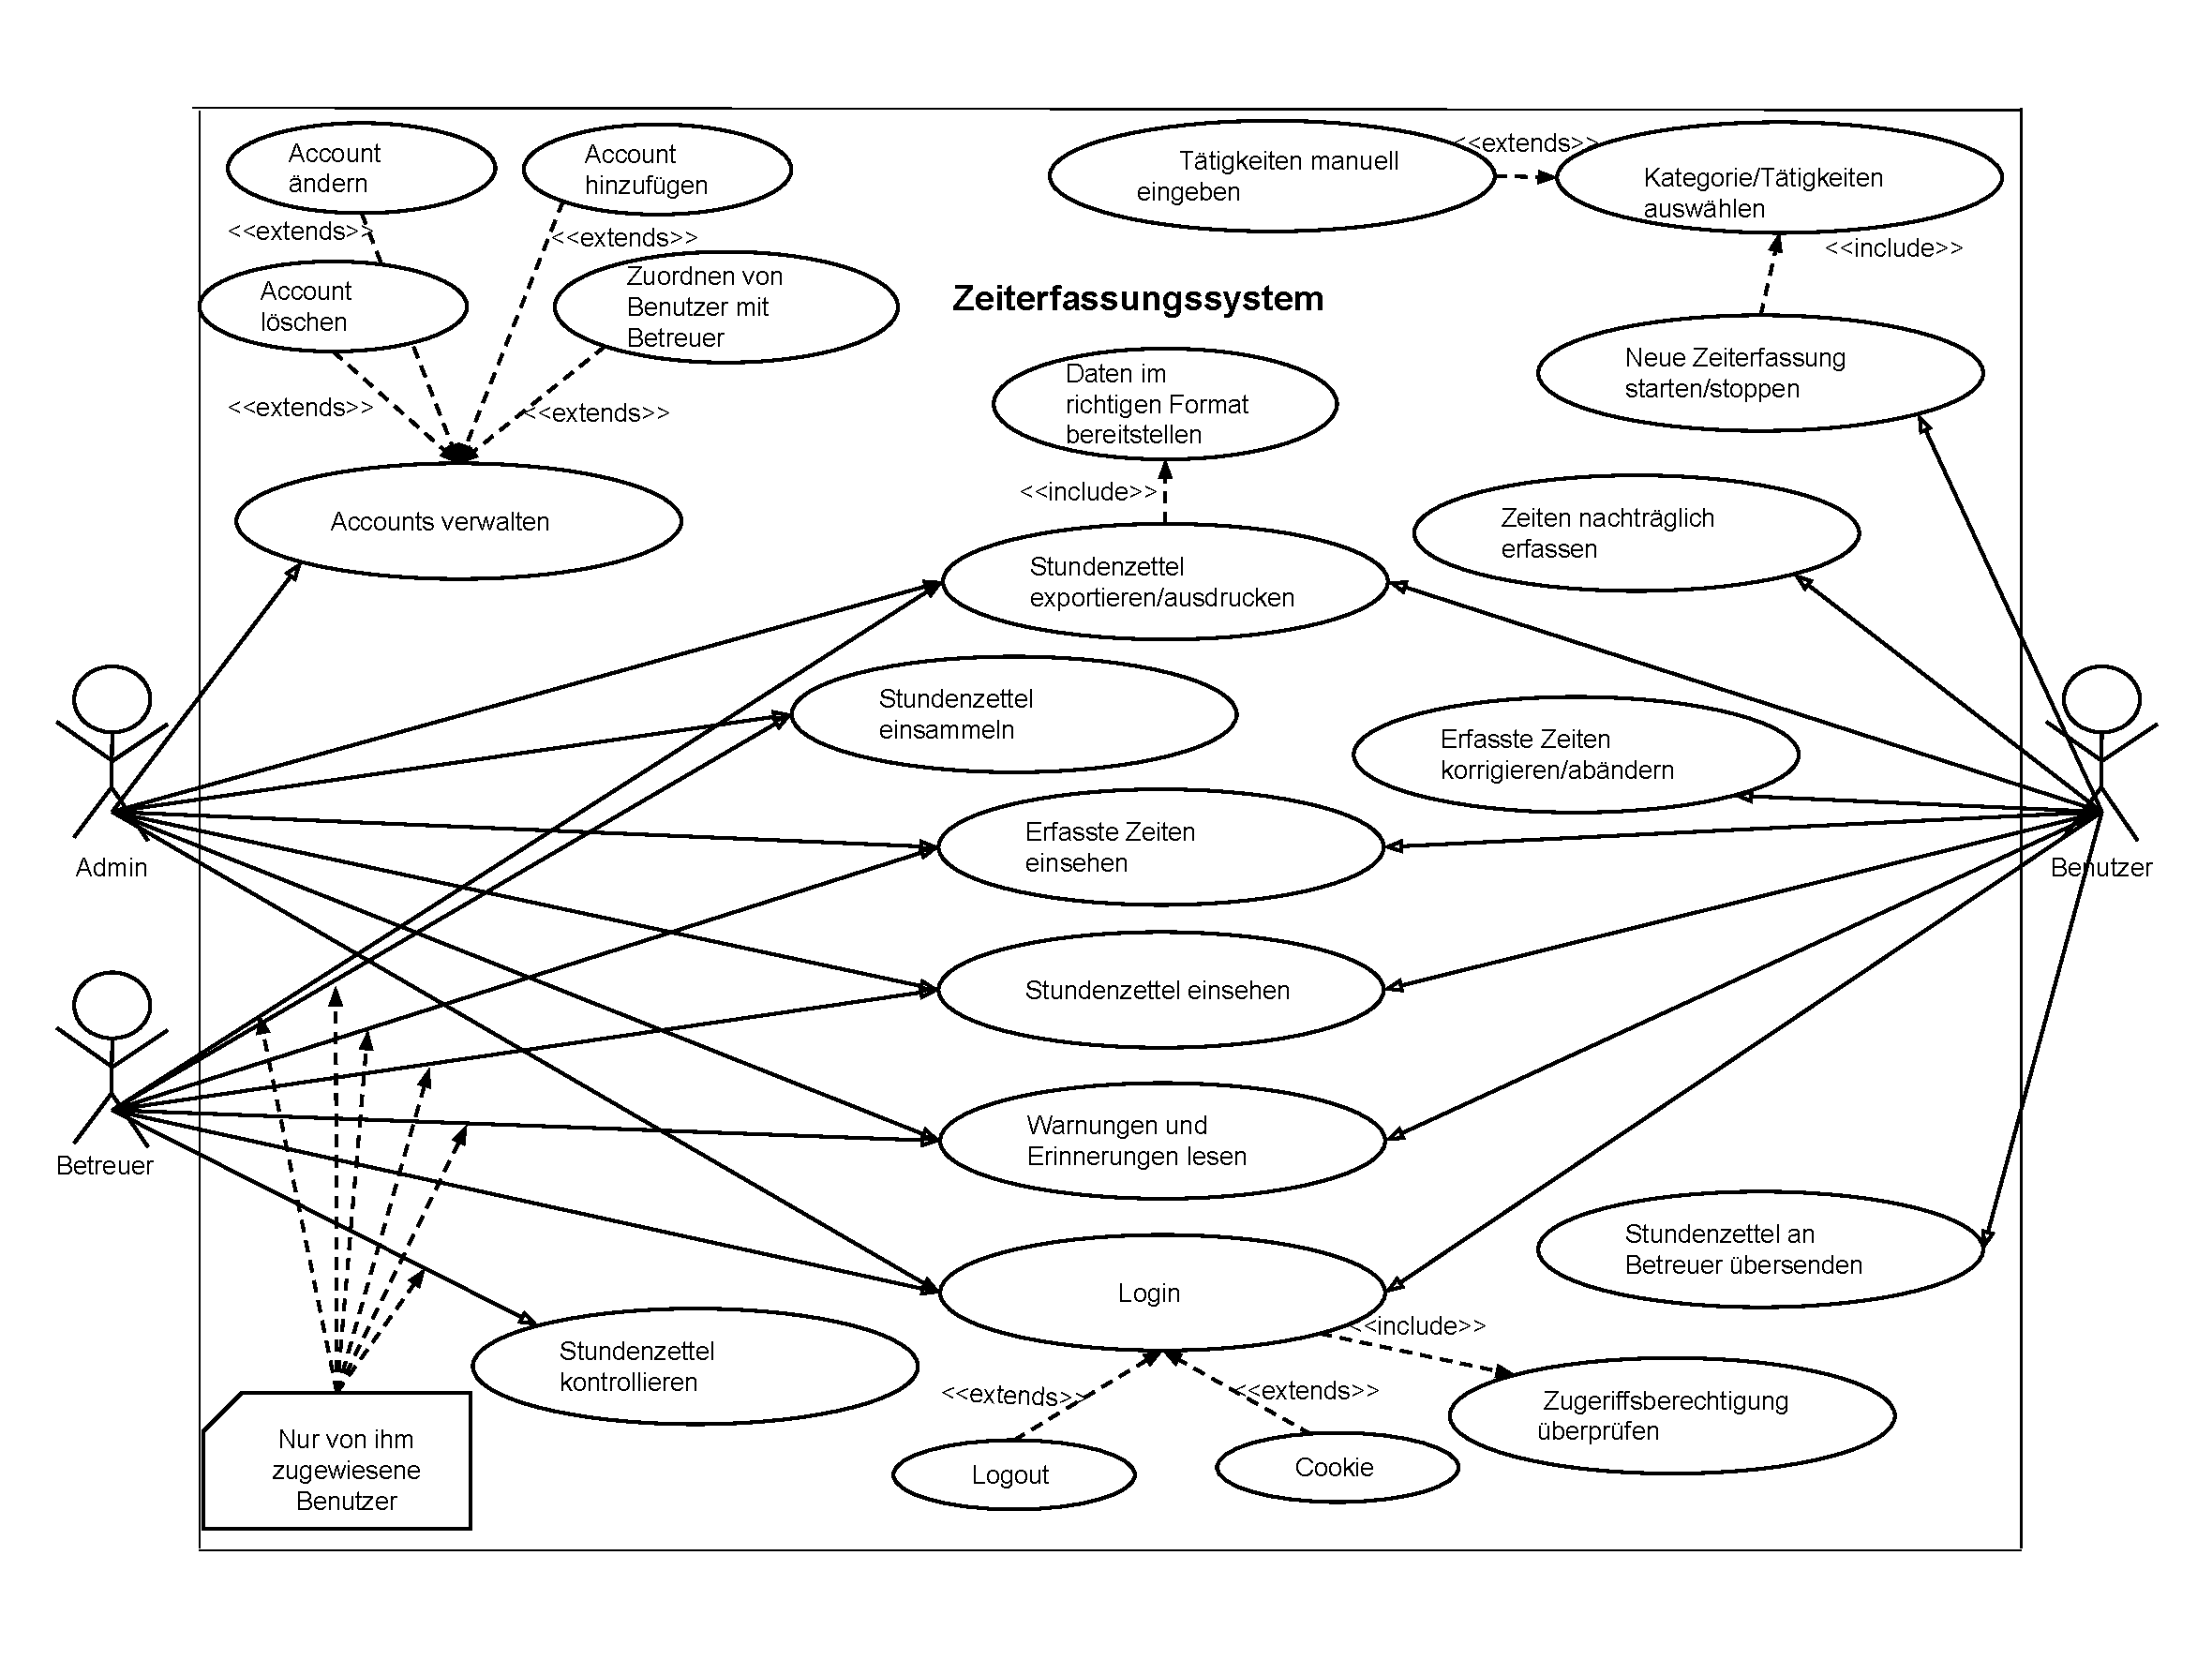
\includegraphics[width=\linewidth]{Anwendungsfalldiagramm.pdf}\\
